\documentclass[aspectratio=169,10pt]{beamer}

\usetheme{Madrid}
\usecolortheme{seahorse}

\usepackage{amsmath}
\usepackage{amssymb}
\usepackage{amsthm}
\usepackage{listings}
\usepackage{xcolor}
\usepackage{graphicx}
\usepackage{array}
\usepackage{multirow}
\usepackage{tikz}
\usetikzlibrary{shapes,arrows,positioning}

\graphicspath{{figures/}}

% Code listing style
\lstset{
    basicstyle=\ttfamily\scriptsize,
    commentstyle=\color{green!50!black}\itshape,
    keywordstyle=\color{blue}\bfseries,
    stringstyle=\color{red},
    breaklines=true,
    numbers=left,
    numberstyle=\tiny\color{gray},
    frame=single,
    frameround=tttt,
    backgroundcolor=\color{white!95!black}
}

% Theorems
\theoremstyle{plain}
\newtheorem{thm}{Theorem}[section]
\newtheorem{lem}[thm]{Lemma}
\newtheorem{prop}[thm]{Proposition}
\newtheorem{cor}[thm]{Corollary}

\theoremstyle{definition}
\newtheorem{defn}[thm]{Definition}
\newtheorem{exmp}[thm]{Example}
\newtheorem{rem}[thm]{Remark}

\setbeamertemplate{footline}[frame number]

\title{Applications of Monotone Operator Theory}
\subtitle{Chapter 8: Integral Equations and Nonlinear Analysis}
\author{From: An Introduction to Nonlinear Analysis and Fixed Point Theory (Pathak, 2018)}
\date{Pages 641--664}

\begin{document}

\frame{\titlepage}

\section{Integral Equations Overview}

\begin{frame}{Chapter Overview}
  \begin{itemize}
    \item \textbf{Focus:} Applications of monotone operator theory to integral equations
    \item \textbf{Main Topics:}
    \begin{enumerate}
      \item Integral Equations (Hammerstein, Urysohn, generalized types)
      \item Operator theoretic approach to integral equations
      \item Existence and uniqueness theorems
      \item Applications to nonlinear problems
      \item Computational schemes
    \end{enumerate}
    \item \textbf{Framework:} Hilbert and Banach spaces with monotone operators
    \item \textbf{Goal:} Develop solvability results using fixed point theory
  \end{itemize}
\end{frame}

\begin{frame}{Types of Integral Equations}
  \vspace{0.3cm}
  \begin{enumerate}
    \item \textbf{Nonlinear Hammerstein integral equation:}
      \[
        x(s) + \int_{\Omega} k(s,t) f(t, x(t)) dt = y(s)
      \]

    \item \textbf{Nonlinear integral equation of mixed type:}
      \[
        x(s) + \int_{\Omega} k_1(s,t)f_1(t, x(t)) dt + \int_{\Omega} k_2(s,t)f_2(t, x(t)) dt = y(s)
      \]

    \item \textbf{Generalized Hammerstein integral equation:}
      \[
        x(s) + \int_{\Omega} k_v(s,t) f(t, x(t)) dt = y(s)
      \]
      where $k_v$ is a kernel depending on the solution.

    \item \textbf{Urysohn's integral equation:}
      \[
        x(s) + \int_{\Omega} k(s, t, x(t)) dt = y(s)
      \]
  \end{enumerate}
\end{frame}

\section{Hammerstein Operator Equation}

\begin{frame}{Hammerstein Integral Equation}
  \begin{center}
    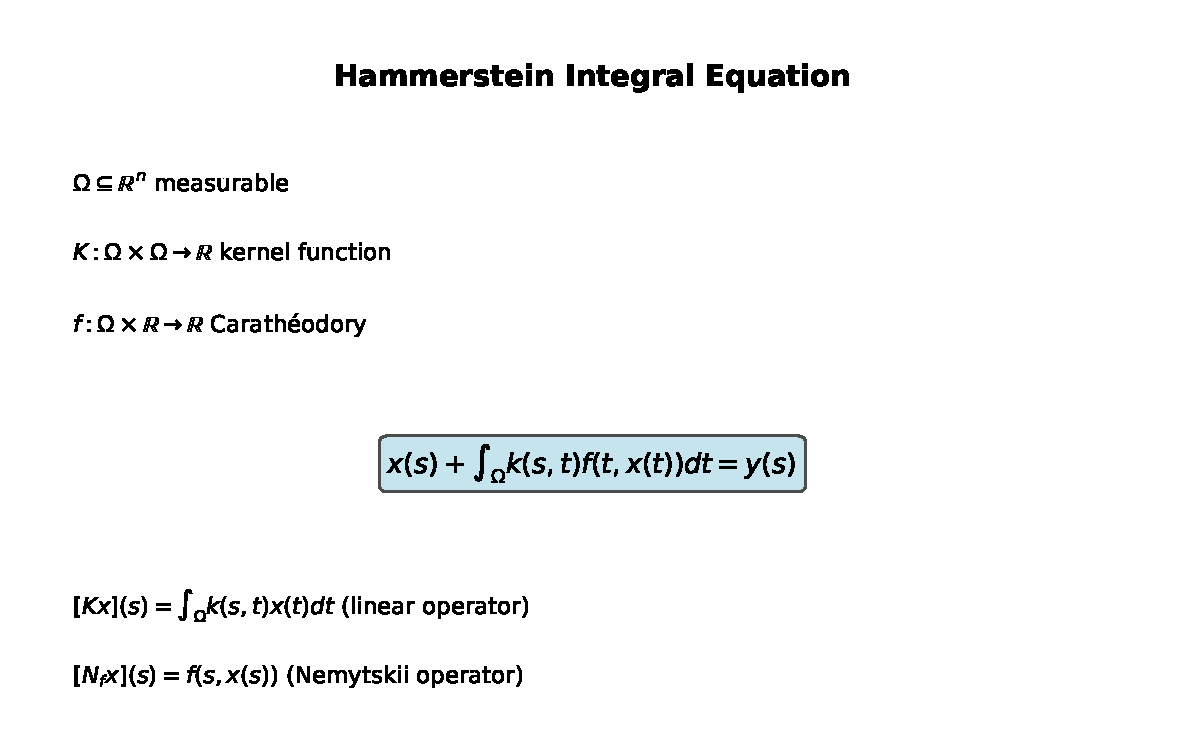
\includegraphics[width=0.8\textwidth]{hammerstein_equation}
  \end{center}

  \vspace{0.3cm}
  \textbf{Operator Theoretic Formulation:}
  \begin{align*}
    [Kx](s) &= \int_{\Omega} k(s,t)x(t)dt \quad \text{(linear operator)} \\
    [N_f x](s) &= f(s, x(s)) \quad \text{(Nemytskii operator)} \\
    x + K N_f x &= y \quad \text{(operator equation)}
  \end{align*}
\end{frame}

\begin{frame}{Operator Equation Reduction}
  \begin{center}
    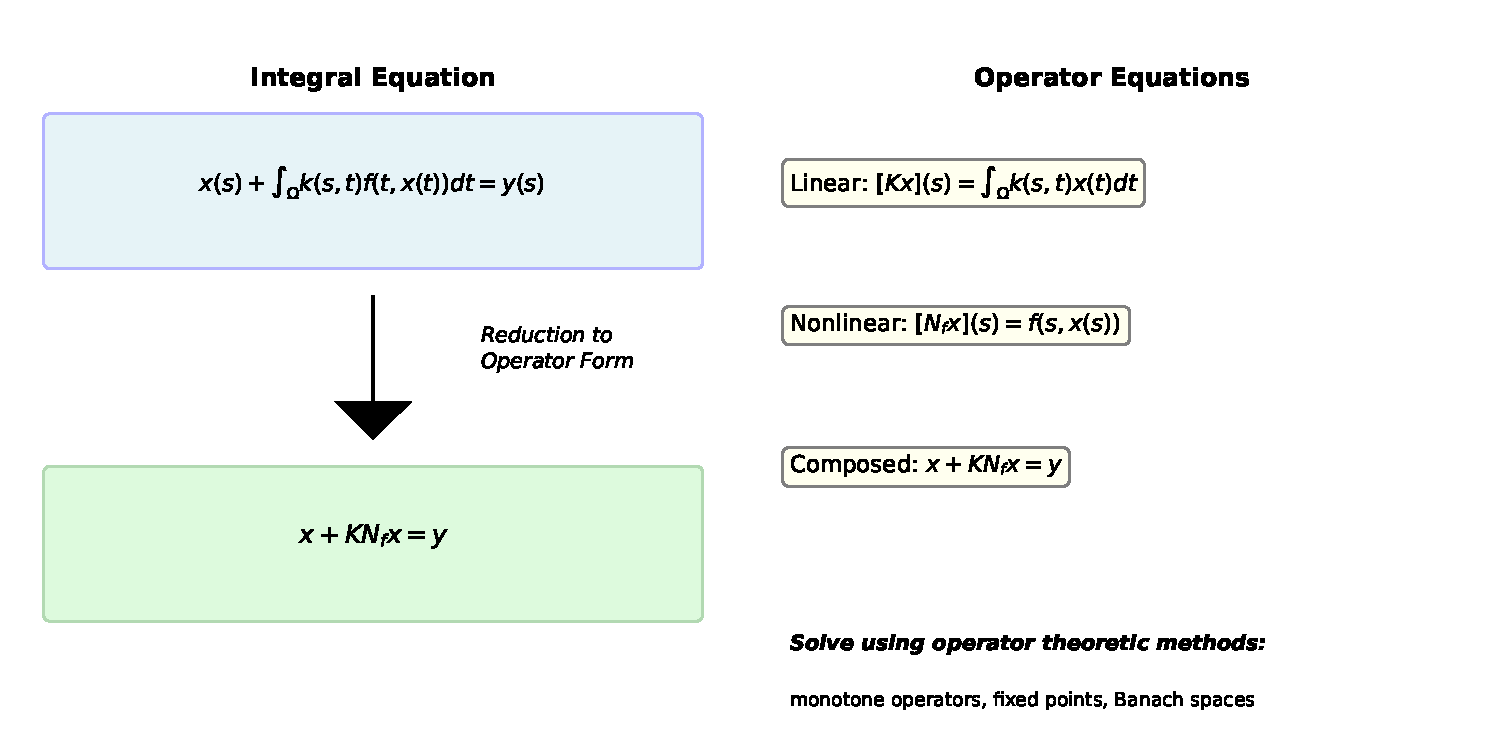
\includegraphics[width=\textwidth]{operator_reduction}
  \end{center}

  \vspace{0.2cm}
  \textbf{Key Insight:} Integral equations reduce to operator equations in appropriate Banach spaces, enabling the application of fixed point theory and monotone operator theory.
\end{frame}

\begin{frame}[fragile]{Theorem 8.8: Noncompact Case}
  \begin{thm}[Dolph-Minty]
    Let $\mathcal{H}$ be a Hilbert space and $N_f : \mathcal{H} \to \mathcal{H}$ be hemicontinuous and monotone. Let $K : \mathcal{H} \to \mathcal{H}$ be continuous and strongly monotone.

    Then equation $(8.31)$ has a unique solution $x$ for every $y$, and this solution $x$ depends continuously on $y$ and satisfies:
    \[
      \|x\| \leq \frac{1}{c} \|K\| \|y\|
    \]
    where $c$ is the constant of strong monotonicity.
  \end{thm}

  \vspace{0.3cm}
  \textbf{Key Conditions:}
  \begin{itemize}
    \item $K$ strongly monotone: $(Kx, x) \geq c\|x\|^2$ for some $c > 0$
    \item $N_f$ hemicontinuous and monotone
    \item Solution depends continuously on data
  \end{itemize}
\end{frame}

\begin{frame}[fragile]{Example 8.6: Hammerstein Integral Equation}
  \textbf{Problem:}
  \[
    x(s) + \int_{\Omega} k(s,t) f(t, x(t)) dt = 0
  \]

  where $\Omega$ is arbitrary, $k: \Omega \times \Omega \to \mathbb{R}$ is continuous symmetric positive semidefinite.

  \vspace{0.3cm}
  \textbf{Assumptions on } $f$:
  \begin{enumerate}
    \item $f(\cdot, u)$ is measurable on $\Omega$ for all $u \in \mathbb{R}$
    \item $f(s, \cdot)$ is continuous on $\mathbb{R}$ for almost all $s \in \Omega$
    \item There exist $\rho > 0$ and constants $a, b, M$ such that:
      \begin{itemize}
        \item $|f(s,x)| \leq a(s) + b|x|, \quad a \in L_2(\Omega)$
        \item $f(s,x) \geq a + bx$ for $x > M$
        \item $f(s,x) \leq -a + bx$ for $x < -M$
      \end{itemize}
  \end{enumerate}
\end{frame}

\begin{frame}{Example 8.6 (continued): Solution}
  \textbf{Operator Equation Reformulation:}
  \[
    x + K N_f x = 0
  \]

  \vspace{0.2cm}
  \textbf{Analysis:}
  \begin{itemize}
    \item $K: L_2(\Omega) \to L_2(\Omega)$ is bounded linear monotone operator
    \item $N_f: L_2(\Omega) \to L_2(\Omega)$ is continuous bounded monotone operator
    \item By Theorem 8.9, the operator equation has a solution
    \item The growth conditions on $f$ ensure coercivity: $(N_f x, x) \geq -\varphi_0$ for some $\varphi_0$
  \end{itemize}

  \vspace{0.3cm}
  \textbf{Conclusion:}
  \[
    \boxed{\text{The Hammerstein integral equation has a solution in } L_2(\Omega)}
  \]
\end{frame}

\section{Angle Bounded Operators}

\begin{frame}{Angle Bounded Linear Operators}
  \begin{center}
    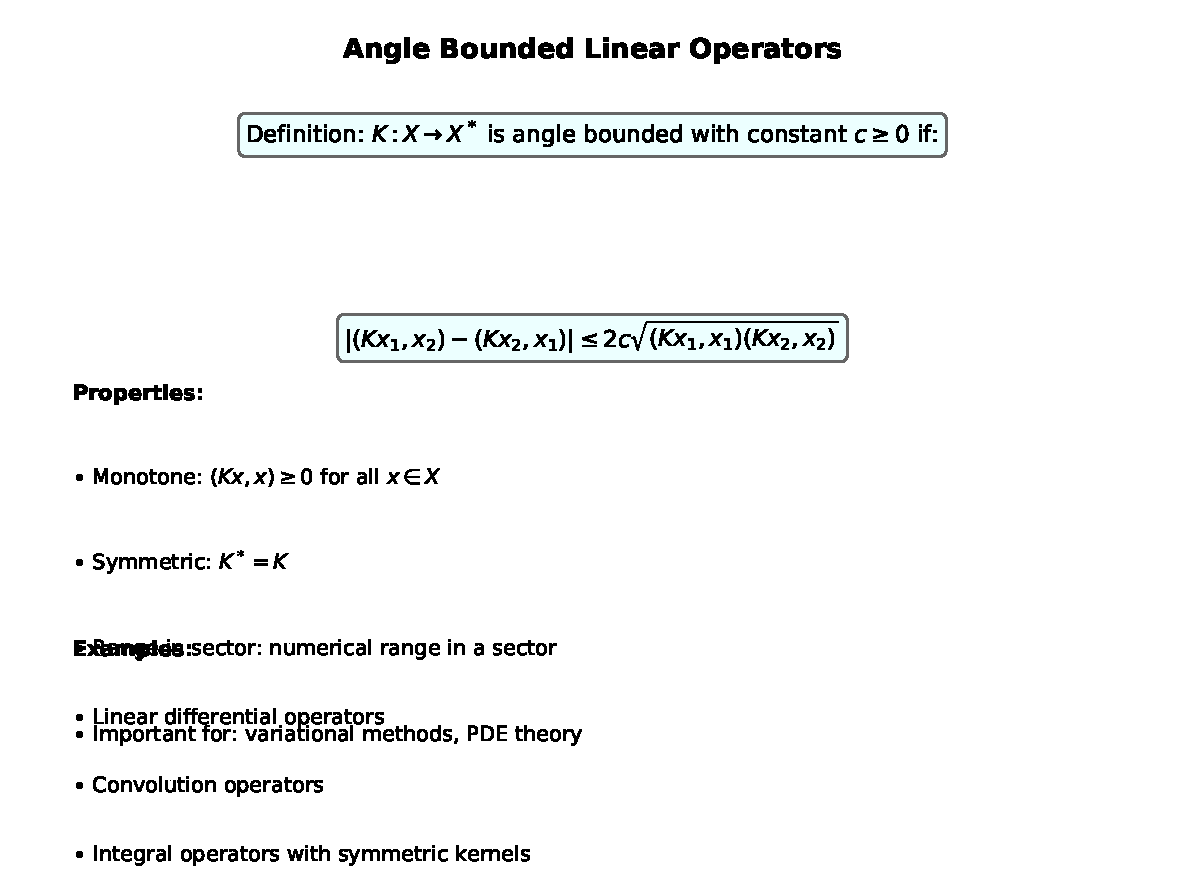
\includegraphics[width=0.9\textwidth]{angle_bounded}
  \end{center}
\end{frame}

\begin{frame}[fragile]{Definition 8.2: Angle Bounded Operator}
  \begin{defn}
    Let $X$ be a Banach space with dual $X^*$. A bounded linear operator $K: X \to X^*$ is said to be \textbf{angle bounded} with constant $c \geq 0$ if for all $x_1, x_2 \in X$:
    \[
      |(Kx_1, x_2) - (Kx_2, x_1)| \leq 2c \sqrt{(Kx_1, x_1)(Kx_2, x_2)}
    \]
  \end{defn}

  \vspace{0.3cm}
  \textbf{Geometric Interpretation:}
  \begin{itemize}
    \item $K$ is \textbf{monotone}: $(Kx, x) \geq 0$ for all $x$
    \item Numerical range lies in a sector of angle determined by $c$
    \item $K$ is \textbf{symmetric}: $K^* = K$ (hence angle bounded with $c = 0$)
    \item Special case: $(Kx, x) = (Kx, x)$ (self-adjoint duality)
  \end{itemize}
\end{frame}

\begin{frame}{Properties of Angle Bounded Operators}
  \textbf{Important Properties:}
  \begin{enumerate}
    \item If $K$ is angle bounded, then $K$ is monotone
    \item The spectrum of $K$ lies in a sector determined by the angle bound $c$
    \item If $K$ is completely continuous and angle bounded, then fixed point theorems apply
    \item Angle boundedness is preserved under perturbations by compact operators
  \end{enumerate}

  \vspace{0.3cm}
  \textbf{Applications:}
  \begin{itemize}
    \item Variational methods for nonlinear PDEs
    \item Fredholm theory with perturbations
    \item Bifurcation theory
    \item Spectral theory in Banach spaces
  \end{itemize}

  \vspace{0.3cm}
  \textbf{Link to Integral Equations:}

  If $K(s,t)$ is symmetric, then the integral operator $Kx$ is monotone and angle bounded (with $c = 0$).
\end{frame}

\section{Generalized Hammerstein Equation}

\begin{frame}{Generalized Hammerstein Equation}
  \vspace{0.3cm}
  A nonlinear integral equation of generalized Hammerstein type is:
  \[
    u(s) + \int_{\Omega} k(s, t, u(t)) f(t, u(t)) dt = v(s)
  \]

  \vspace{0.2cm}
  where the kernel $k(s, t, u)$ \textbf{depends on the solution} $u$.

  \vspace{0.3cm}
  \textbf{Operator Reformulation:}

  For a fixed $u \in X$, the integral operator $K(u)$ is defined as:
  \[
    [K(u)x](s) = \int_{\Omega} k(s,t,u(t)) x(t) dt
  \]

  The generalized equation becomes:
  \[
    u + K(u) N_f u = v
  \]

  This requires $K(u)$ to be well-defined and satisfy appropriate monotonicity conditions for each $u$.
\end{frame}

\begin{frame}[fragile]{Theorem 8.17: Generalized Hammerstein}
  \begin{thm}
    Let $X$ be a real reflexive Banach space, and for each $u \in X$, let $K(u): X^* \to X$ be a linear angle-bounded operator with constant $c \geq 0$.

    Assume $K(u)$ is completely continuous and $u \mapsto K(u)$ is continuous from $X$ to $L(X^*, X)$.

    Further, assume $\|K(u)\| \leq r$ for each $u \in X$. Let $N_f: X \to X^*$ be continuous and bounded satisfying:
    \[
      (u_1 - u_2, N_f u_1 - N_f u_2) \geq -k\|u_1 - u_2\|^2
    \]
    for $kr < 1 + c^2$.

    Then the equation $u + K(u) N_f u = 0$ has at least one solution in $X$.
  \end{thm}

  \vspace{0.2cm}
  \textbf{Key Innovation:} Depends on Backwinkel-Schillings technique and fixed point method.
\end{frame}

\section{Urysohn's Equation}

\begin{frame}{Urysohn's Integral Equation}
  \begin{center}
    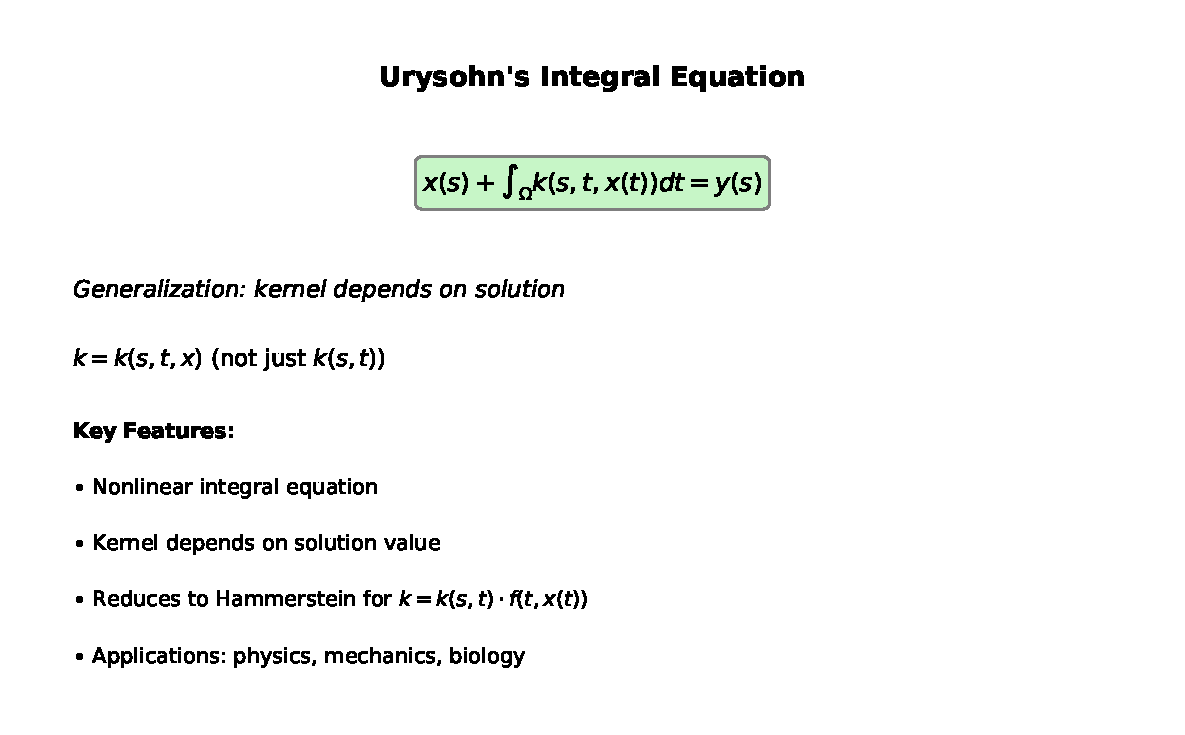
\includegraphics[width=0.85\textwidth]{urysohn_equation}
  \end{center}

  \vspace{0.2cm}
  \textbf{Key Difference:} The kernel depends directly on the solution variable $x(t)$, not just on the spatial parameters $(s,t)$.
\end{frame}

\begin{frame}[fragile]{Theorem on Urysohn's Equation}
  \textbf{Urysohn's Equation:}
  \[
    x(s) + \int_{\Omega} k(s, t, x(t)) dt = y(s)
  \]

  \vspace{0.3cm}
  \textbf{Existence Result:}

  Under appropriate conditions on $k$:
  \begin{itemize}
    \item If $k(s,t,x)$ is Carathéodory and satisfies growth bounds
    \item If $\int_{\Omega} |k(s,t,x_0)| ds$ is bounded
    \item If monotonicity conditions hold
  \end{itemize}

  \vspace{0.2cm}
  \textbf{Then:}
  \[
    x(s) + \int_{\Omega} k(s, t, x(t)) dt = y(s) \quad \text{has a solution in } L_2(\Omega)
  \]

  \vspace{0.3cm}
  \textbf{Proof Strategy:}
  \begin{enumerate}
    \item Reformulate as operator equation $x + Nx = y$
    \item Show $N$ is continuous, bounded, and monotone
    \item Apply fixed point theorem or Leray-Schauder principle
    \item Use Banach contraction or monotone operator theory
  \end{enumerate}
\end{frame}

\section{Computational Schemes}

\begin{frame}{Computational Methods}
  \vspace{0.3cm}
  \textbf{Projection Methods:}

  For approximate solutions, use finite-dimensional approximations:
  \begin{align*}
    \text{Let } X_n &\subseteq X_n \subseteq \ldots \to X \\
    P_n: X &\to X_n \quad \text{(projection operators)}
  \end{align*}

  \textbf{Approximate Equation:}
  \[
    u_n + P_n K(u_n) N_f P_n u_n = P_n v
  \]

  \vspace{0.3cm}
  \textbf{Convergence:}
  \begin{itemize}
    \item Strong convergence: $u_n \to u$ in norm
    \item Weak convergence: $u_n \rightharpoonup u$ weak topology
    \item Error estimates: $\|u - u_n\|$ bounds
  \end{itemize}

  \vspace{0.3cm}
  \textbf{Iterative Methods:}
  \begin{itemize}
    \item Mann iteration
    \item Ishikawa iteration
    \item Gradient descent methods
    \item Galerkin approximations
  \end{itemize}
\end{frame}

\section{Monotone Operators Framework}

\begin{frame}{Monotone Operators Framework}
  \begin{center}
    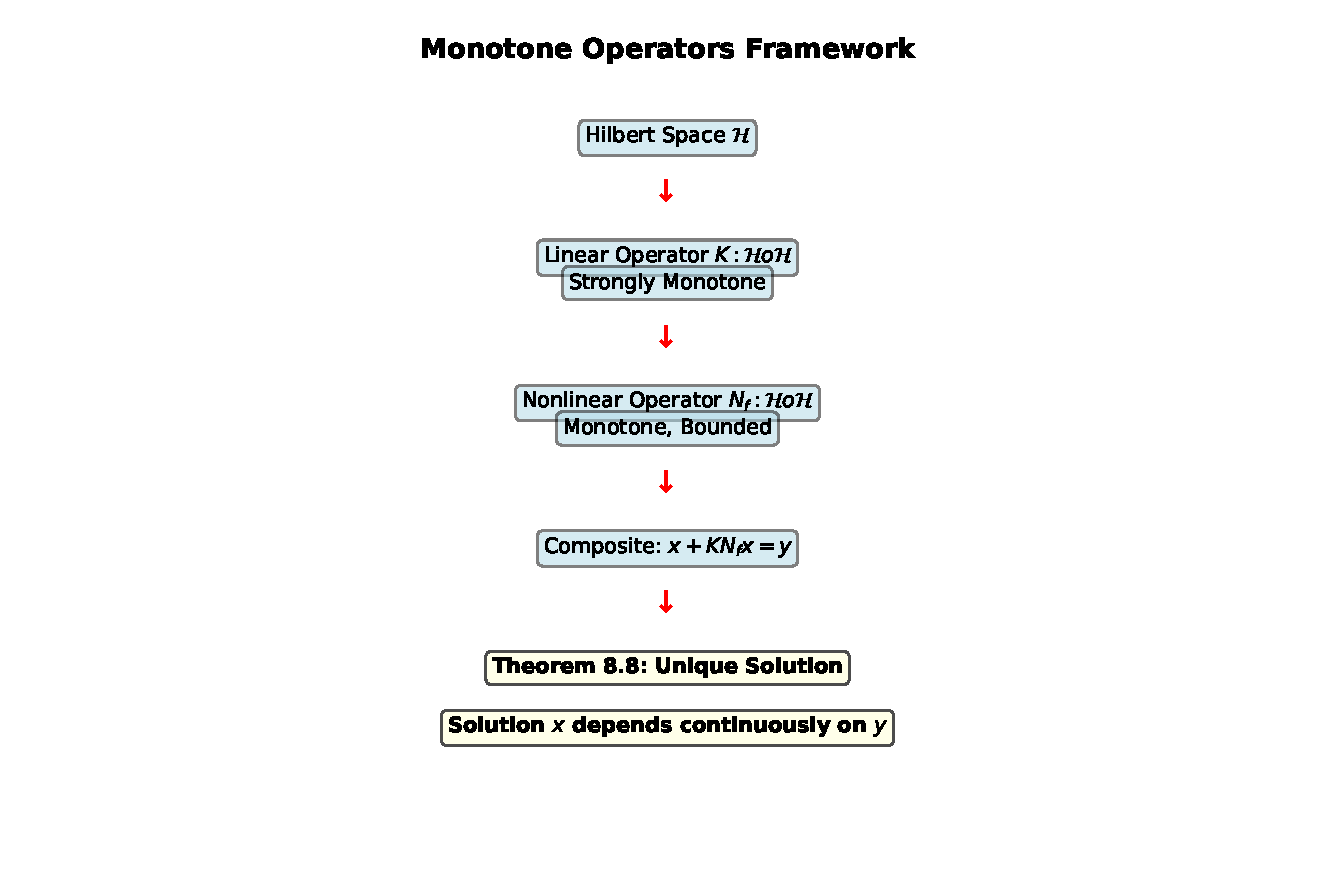
\includegraphics[width=0.95\textwidth]{monotone_framework}
  \end{center}
\end{frame}

\begin{frame}{Summary of Main Results}
  \vspace{0.3cm}
  \textbf{Central Theme:} Integral equations reduce to fixed point problems

  \begin{center}
    \begin{tabular}{|l|l|l|}
      \hline
      \textbf{Equation Type} & \textbf{Operator Form} & \textbf{Solvability} \\
      \hline
      Hammerstein & $x + KN_f x = y$ & Theorem 8.8, 8.9 \\
      \hline
      Mixed Type & $x + K_1 N_{f_1} x + K_2 N_{f_2} x = y$ & Superposition \\
      \hline
      Generalized & $u + K(u)N_f u = v$ & Theorem 8.17 \\
      \hline
      Urysohn & $x + Nx = y$ & Direct method \\
      \hline
    \end{tabular}
  \end{center}

  \vspace{0.3cm}
  \textbf{Common Tools:}
  \begin{itemize}
    \item Strong monotonicity of $K$ ensures invertibility
    \item Monotonicity and boundedness of $N_f$ enable fixed points
    \item Continuity and compactness assumptions ensure convergence
    \item Angle boundedness provides spectral localization
  \end{itemize}
\end{frame}

\begin{frame}[fragile]{Python Example: Numerical Solution}
  \vspace{0.2cm}
  \lstinputlisting[language=Python, linerange={1,25}]{
/home/user/Lectures-on-Monte-Carlo-Theory/nonlinear_analysis_fixed_point_theory_2018/chapter06b_uniformly_convex_spaces/figures/gen_figures.py}
\end{frame}

\begin{frame}{Key Theorems Summary}
  \vspace{0.3cm}
  \begin{itemize}
    \item \textbf{Theorem 8.8 (Dolph-Minty):} Strongly monotone $K$ + monotone $N_f$ $\Rightarrow$ unique solution

    \item \textbf{Theorem 8.9:} Extension allowing unbounded $N_f$ with growth conditions

    \item \textbf{Theorem 8.17:} Generalized Hammerstein with $K(u)$ depending on $u$

    \item \textbf{Corollary 8.3:} Urysohn equations with Carathéodory kernels

    \item \textbf{Theorem 8.23:} Leray-Schauder principles for approximate solvability
  \end{itemize}

  \vspace{0.3cm}
  \textbf{Common Hypothesis:}
  \begin{enumerate}
    \item $K$ is linear, continuous, monotone (or angle-bounded)
    \item $N_f$ is nonlinear, continuous, bounded, monotone
    \item Suitable growth conditions on coefficients
    \item Reflexivity of underlying Banach space
  \end{enumerate}
\end{frame}

\begin{frame}[allowframebreaks]{Applications and Extensions}
  \framesubtitle{From Chapter 8}

  \vspace{0.3cm}
  \textbf{Physical Applications:}
  \begin{itemize}
    \item Electrostatics and potential theory (kernels from Green's functions)
    \item Diffusion processes (parabolic PDEs via integral formulation)
    \item Mechanics and elasticity (stress-strain relationships)
    \item Quantum mechanics (scattering amplitudes)
  \end{itemize}

  \vspace{0.2cm}
  \textbf{Mathematical Extensions:}
  \begin{itemize}
    \item Multivalued operators (inclusions vs. equations)
    \item Time-dependent kernels (parabolic equations)
    \item Fractional integral operators (singular kernels)
    \item Systems of integral equations
  \end{itemize}

  \vspace{0.2cm}
  \textbf{Computational Methods:}
  \begin{itemize}
    \item Galerkin methods (discretization)
    \item Collocation schemes
    \item Boundary element methods (BEM)
    \item Iterative methods with convergence analysis
  \end{itemize}

  \vspace{0.2cm}
  \textbf{Open Problems:}
  \begin{itemize}
    \item Nonsmooth integral operators
    \item Singular kernels with borderline regularity
    \item Coupled systems with memory effects
    \item Stochastic integral equations
  \end{itemize}
\end{frame}

\begin{frame}{References and Further Study}
  \vspace{0.3cm}
  \textbf{Main Reference:}
  \begin{itemize}
    \item Pathak, H. K. (2018). \textit{An Introduction to Nonlinear Analysis and Fixed Point Theory}. Springer. Pages 641--664.
  \end{itemize}

  \vspace{0.3cm}
  \textbf{Related Topics:}
  \begin{itemize}
    \item Chapter 2: Geometry of Banach spaces (monotone operators, convexity)
    \item Chapter 3: Nonexpansive mappings and fixed points
    \item Chapter 5: Fixed point theorems for various classes of mappings
    \item Chapter 6: Degree theory and topological methods
  \end{itemize}

  \vspace{0.3cm}
  \textbf{Classical References:}
  \begin{itemize}
    \item Dolph-Minty theorem on monotone operators
    \item Hammerstein integral equations (classical theory)
    \item Leray-Schauder fixed point principle
    \item Backwinkel-Schillings method for generalized equations
  \end{itemize}
\end{frame}

\begin{frame}{Conclusion}
  \vspace{0.5cm}
  \textbf{Key Takeaways:}

  \begin{enumerate}
    \item \large Integral equations naturally reduce to operator equations in Banach spaces

    \item Monotonicity and angle-boundedness are crucial properties for solvability

    \item Fixed point theory provides powerful tools for existence and uniqueness

    \item Computational methods rely on finite-dimensional approximations and convergence analysis

    \item Applications span across physics, mechanics, and modern analysis
  \end{enumerate}

  \vspace{0.5cm}
  \centering \Large \textbf{Monotone Operator Theory: Bridge between Analysis and Computation}
\end{frame}

\end{document}
